\chapter{Sensor fusion controlling}
\label{chap:SensFusContr}

To achieve the statistical data of all sensors of the inertial measurement unit a Matlab model is used. This model also helps to check the results of the two different fusion filters, the Kalman filter and the complementary filter. The data is send via UDP-packets from the Raspberry Pi to the Matlab model on the Host computer. Figure \ref{fig:model} shows the used Matlab model. Additional a 3D representation of the rotations is visualized and can be directly compared with the integrated offset corrected gyroscope data.

\begin{figure}[H]
	\centering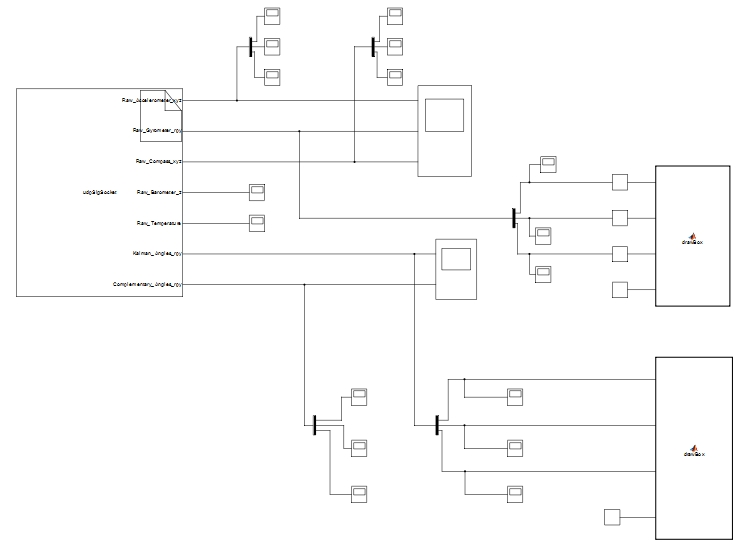
\includegraphics[width=1\textwidth]{fig/Model}
	\caption{Matlab model}
	\label{fig:model}
\end{figure}

\newpage
With the help of the scopes within this model, the logged data is stored in the Matlab workspace and then it is analyzed with a Matlab file. With the help of this file, a histogram from every sensor is generated. Also the meanvalue and the variance from those sensor is calculated. Finally a plot from the complementary filter and Kalman filter is generated. Also the needed minmum and maximum values of the magnetic sensor is stored. This needs to be done to reduce the influences of hard magnetic parts to the magnetic sensor. Those stored minmium and maximum values are then written in a header file (OrientationDefines.h) which needs to be copied to the folder of the Orientation.c and Orientation.h files. To achieve the best performance, the description of chapter \ref{chap:angle} needs to be followed.

\lstset{language=Matlab,%
backgroundcolor=\color{white}  
}

\begin{lstlisting}
headerFileName = 'OrientationDefines.h';

%Acceleration sensor
figure(1)
%plot histogram of ax and calculate meanvalue and variance
subplot(3,1,1)
hist(ax.signals.values(:),50);
    M=mean(ax.signals.values(:));
    V=var(ax.signals.values(:));
title('Acceleration sensor')
disp(['Meanvalue: ' num2str(M)])
xlabel({'Raw data of sensor ax' ['Mean: ' num2str(M)] ['Varianz: ' num2str(V)]}) % x-axis label

%plot histogram of ay and calculate meanvalue and variance
subplot(3,1,2)
hist(ay.signals.values(:),50);
    M=mean(ay.signals.values(:));
    V=var(ay.signals.values(:));
xlabel({'Raw data of sensor ay' ['Mean: ' num2str(M)] ['Varianz: ' num2str(V)]}) % x-axis label
ylabel('Count of appearance') % y-axis label

%plot histogram of az and calculate meanvalue and variance
subplot(3,1,3)
hist(az.signals.values(:),50);
    M=mean(az.signals.values(:));
    V=var(az.signals.values(:));
xlabel({'Raw data of sensor az' ['Mean: ' num2str(M)] ['Varianz: ' num2str(V)]}) % x-axis label

%Magnetic sensor
figure(2)
%plot histogram of mx and calculate meanvalue and variance
subplot(3,1,1)
hist(mx.signals.values(:),50);
    M=mean(mx.signals.values(:));
    V=var(mx.signals.values(:));
title('Magnetic sensor')
disp(['Meanvalue: ' num2str(M)])
xlabel({'Raw data of sensor mx' ['Mean: ' num2str(M)] ['Varianz: ' num2str(V)]}) % x-axis label

%plot histogram of my and calculate meanvalue and variance
subplot(3,1,2)
hist(my.signals.values(:),50);
    M=mean(my.signals.values(:));
    V=var(my.signals.values(:));
xlabel({'Raw data of sensor my' ['Meanvalue: ' num2str(M)] ['Varianz: ' num2str(V)]}) % x-axis label
ylabel('Count of appearance') % y-axis label

%plot histogram of mz and calculate meanvalue and variance
subplot(3,1,3)
hist(mz.signals.values(:),50);
    M=mean(mz.signals.values(:));
    V=var(mz.signals.values(:));
xlabel({'Raw data of sensor mz' ['Meanvalue: ' num2str(M)] ['Variance: ' num2str(V)]}) % x-axis label

%Gyroscope sensor
figure(3)
%plot histogram of pitch and calculate meanvalue and variance
subplot(3,1,1)
hist(pitch.signals.values(:),50);
    M=mean(pitch.signals.values(:));
    V=var(pitch.signals.values(:));
title('Gyroscope sensor')
disp(['Meanvalue: ' num2str(M)])
xlabel({'Raw data of sensor pitch rate' ['Mean: ' num2str(M)] ['Varianz: ' num2str(V)]}) % x-axis label

%plot histogram of roll and calculate meanvalue and variance
subplot(3,1,2)
hist(roll.signals.values(:),50);
    M=mean(roll.signals.values(:));
    V=var(roll.signals.values(:));
xlabel({'Raw data of sensor roll rate' ['Meanvalue: ' num2str(M)] ['Varianz: ' num2str(V)]}) % x-axis label
ylabel('Count of appearance') % y-axis label

%plot histogram of yaw and calculate meanvalue and variance
subplot(3,1,3)
hist(yaw.signals.values(:),50);
    M=mean(yaw.signals.values(:));
    V=var(yaw.signals.values(:));
xlabel({'Raw data of sensor yaw rate' ['Meanvalue: ' num2str(M)] ['Variance: ' num2str(V)]}) % x-axis label


%Complementary filter
figure(4)
subplot(3,1,1)
plot(Comp_pitch.time,Comp_pitch.signals.values(:));
title('Complementary filter')
xlabel('time [s]') % x-axis label
ylabel('pitch [degree]') % y-axis label

subplot(3,1,2)
plot(Comp_roll.time,Comp_roll.signals.values(:));
xlabel('time [s]') % x-axis label
ylabel('roll [degree]') % y-axis label

subplot(3,1,3)
plot(Comp_yaw.time,Comp_yaw.signals.values(:));
xlabel('time [s]') % x-axis label
ylabel('yaw [degree]') % y-axis label


%Kalman filter
figure(5)
subplot(3,1,1)
plot(Kalman_pitch.time,Kalman_pitch.signals.values(:));
title('Kalman filter')
xlabel('time [s]') % x-axis label
ylabel('pitch [degree]') % y-axis label

subplot(3,1,2)
plot(Kalman_roll.time,Kalman_roll.signals.values(:));
xlabel('time [s]') % x-axis label
ylabel('roll [degree]') % y-axis label

subplot(3,1,3)
plot(Kalman_yaw.time,Kalman_yaw.signals.values(:));
xlabel('time [s]') % x-axis label
ylabel('yaw [degree]') % y-axis label

%min max of magnetic sensor
maxz=max(mz.signals.values)*1000000;
minz=min(mz.signals.values)*1000000;
maxy=max(my.signals.values)*1000000;
miny=min(my.signals.values)*1000000;
maxx=max(mx.signals.values)*1000000;
minx=min(mx.signals.values)*1000000;

fprintf('\n');
disp('Calibration Data:');
disp('=================');
disp(['Min_X: ' num2str(minx)])
disp(['Max_X: ' num2str(maxx)])
disp(['Min_Y: ' num2str(miny)])
disp(['Max_Y: ' num2str(maxy)])
disp(['Min_Z: ' num2str(minz)])
disp(['Max_Z: ' num2str(maxz)])
fprintf('\n');

disp('==================================');
disp('Generating Calibration-Header-File');
disp('==================================');

disp(['Writing header ', headerFileName, ' ...' ]);
fileID = fopen(headerFileName,'w');
fprintf(fileID,'/*!\n');
fprintf(fileID,' * \\file OrientationDefines.h\n');
fprintf(fileID,' */\n');
fprintf(fileID,'\n');
fprintf(fileID,'#ifndef SIG_ORIENTATION_ORIENTATIONDEFINES_H_\n');
fprintf(fileID,'#define SIG_ORIENTATION_ORIENTATIONDEFINES_H_\n');
fprintf(fileID,'\n');
fprintf(fileID,'//Defines for Acceleration Magnetic angle calculation (automatic calibration via MATLAB)\n');
fprintf(fileID,'#define M_SIGORI_MAG_MINX_F64	%.9f\n',minx);
fprintf(fileID,'#define M_SIGORI_MAG_MAXX_F64	%.9f\n',maxx);
fprintf(fileID,'#define M_SIGORI_MAG_MINY_F64	%.9f\n',miny);
fprintf(fileID,'#define M_SIGORI_MAG_MAXY_F64	%.9f\n',maxy);
fprintf(fileID,'#define M_SIGORI_MAG_MINZ_F64	%.9f\n',minz);
fprintf(fileID,'#define M_SIGORI_MAG_MAXZ_F64	%.9f\n',maxz);
fprintf(fileID,'\n');
fprintf(fileID,'#endif /* SIG_ORIENTATION_ORIENTATIONDEFINES_H_ */\n');
fclose(fileID);
disp('Done');
fprintf('\n');
disp('Calibration successfully processed.');

\end{lstlisting}